\documentclass{article}
% ---------------------- Stuff that should be first
\author{Tyler Ryan}
\title{\booktitle}
\date{January 31, 2023}                             % Only use this if you don't want the date to change


% ---------------------- Packages
\usepackage[margin=2cm]{geometry}
\usepackage{lipsum}                                 % Like blindtext
\usepackage{hyperref}                               % href etc
\usepackage{graphicx}                               % To add pictures
\graphicspath{{./assets/}}                          % Where will your pictures be?
\usepackage{wrapfig}                                % Wrapping Pictures
\usepackage{listings}
\usepackage{fancyhdr}                               % Create headers
\usepackage{indentfirst}                            % Ensures fisrt paragraph after Header is indented
\usepackage{color}                                  % Colored text
\usepackage{tikz, tcolorbox}                        % Colored boxes
\usepackage{environ}
% \usepackage{minted}                               % Requires pdflatex --shell-escape

% ---------------------- Variables/Macros
\newcommand\booktitle{\LaTeX: A Basic Overview}     % Like a Variable
\newcommand\red[1]{{\color{red} #1}}                % Quick way to color text red
% \ns{} == \section*{}
\newcommand\ns[1]{\section*{#1}}                    % A function that takes in 1 parameter
\newtcolorbox{basicbox}[2]{
    colframe = #1,
    title    = #2,
    }

% ---------------------- Environments
% \newenvironment{codeblock}{}{}
% ---------------------- Document
\begin{document}
\pagestyle{fancy}
\fancyhead{}
\fancyhead[REO]{\booktitle}                         % REO == Right, Even, Odd
\fancyhead[LEO]{Noob Central}                       % REO == Right, Even, Odd
\fancyfoot{}
\fancyfoot[REO]{\thepage}
\maketitle
\tableofcontents
\newpage
% \raggedright % Try it

\section{Font Weights}
% This is all 1 line
This section is mainly \textbf{to be used}
\textit{when figuring out how to} \underline{apply weights to text}
\emph{Please \textbf{NOTE} that ''\textbackslash textit'' is only used
when the text is only ever supposed to be underlined} 

\noindent
\textbf{If you mean to emphasise text, then use ''\textbackslash emph''
instead.} 
It is also good to note that to use proper '''' marks, you must actually
use two '' ' ''s.
''This is a quotation''
%------------------------------

% \section*{Labels and References}                                    % section*{} removes the number at the front
\ns{Labels and References}                                    % section*{} removes the number at the front
% See \newcommand\red to see how I did this.
\red{Let's say you want to reference Section 2 (Lists).} 
So you say something like ''just like how it was done in 
section 2 Lists''. However, what if you then change the 
positioning of section 2 Lists and the result is that it 
is now section 3 lists? Then you would have to find ever where
in your document where you referenced "Section 2 Lists" and 
rename it.

\noindent
Let's fix that with \textbackslash label and \textbackslash ref.
and reference Lists in section \ref{lists}. Aha! See what I did
there? No matter where Section \ref{lists} moves to, it 
will always be referened correctly!

\noindent
\textbf{Note}: You will have to compile twice. Upon the first
compilation, there will a \emph{??} in place of the actual 
number.                                                             

\noindent
This is also nice when referencing things in lists. I don't know
which number ''Bread'' might be when the final version of this 
is complete, but I can reference it here: \ref{bread}. Well,
check for your self. Is Bread in part \ref{bread} of Ordered Lists,
which by the way is in \textbf{section \ref{ord-lists}}.

\section{Lists\label{lists}}
    \subsection{Ordered Lists\label{ord-lists}}
        \begin{enumerate}
            \item Bread\label{bread}
            \item Butter
        \end{enumerate}
    \subsection{Non Ordered Lists}
        \begin{itemize}
            \item one
            \item two
        \end{itemize}
    % \newpage
    \subsection{Nested Lists}
        \begin{enumerate}
            \item dog
                \begin{enumerate}
                    \item big dog
                    \item small dog
                \end{enumerate}
            \item cat
                \begin{itemize}
                    \item Loud cat
                    \item Quiet Cat
                \end{itemize}
        \end{enumerate}

\section{Images}
    \subsection{Non Wrapped}
    \lipsum[1-1]
    \begin{figure}[h]
        \centering
        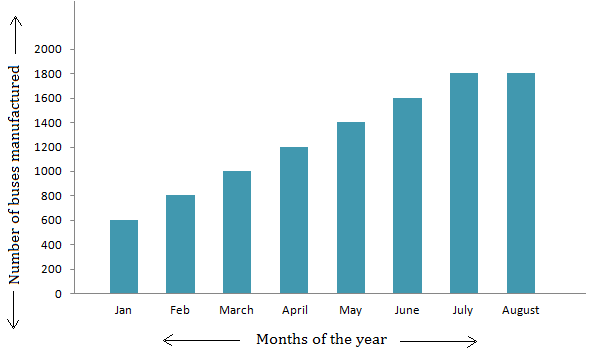
\includegraphics[width=0.90\textwidth]{bar-graph}
        % 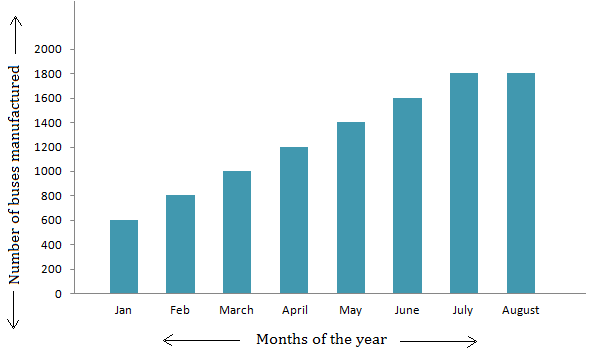
\includegraphics[scale=0.5]{bar-graph}
        \caption{No Wrap Image}
    \end{figure}
    % \newpage
    \subsection{Wrapped}

    % \indent Will not work on the fist line.
    % Instead, \usepackage{indentfirst} does the trick
    This is how you would wrap text around the picture.
    However, I can't seem to get it to work. It would require
    a lot more knowledge about {\LaTeX} to fix than I 
    currently have.
    \lipsum[1-1]

    \begin{wrapfigure}{r}{0.35\textwidth}
        % \vspace*{-6cm}
        \centering
        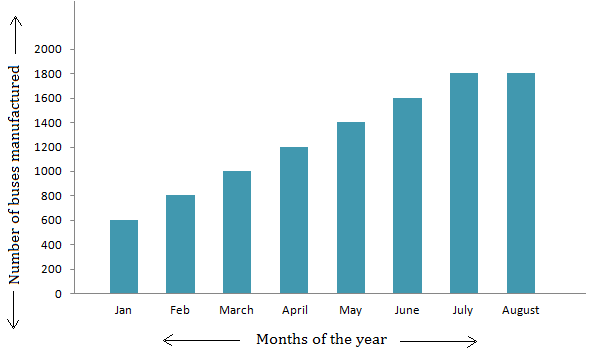
\includegraphics[width=0.35\textwidth]{bar-graph}
      \caption{Image Wrapped to the Right}
    \end{wrapfigure}

    \textbf{This is how you would wrap text around the picture.}

    However, I can't seem to get it to work. It would require
    a lot more knowledge about {\LaTeX} to fix than I 
    currently have. This is how you would wrap text around the picture.
    However, I can't seem to get it to work. It would require
    a lot more knowledge about {\LaTeX} to fix than I currently have.
    This is how you would wrap text around the picture. However, I 
    can't seem to get it to work. It would require
    a lot more knowledge about {\LaTeX} to fix than I 
    currently have.
    This is how you would wrap text around the picture.
    However, I can't seem to get it to work. It would require
    a lot more knowledge about {\LaTeX} to fix than I 
    currently have. This is how you would wrap text around the picture.
    However, I can't seem to get it to work. It would require
    a lot more knowledge about {\LaTeX} to fix than I currently have.
    This is how you would wrap text around the picture. However, I 
    can't seem to get it to work. It would require
    a lot more knowledge about {\LaTeX} to fix than I 
    currently have.
    This is how you would wrap text around the picture.
    However, I can't seem to get it to work. It would require
    a lot more knowledge about {\LaTeX} to fix than I 
    currently have. This is how you would wrap text around the picture.
    However, I can't seem to get it to work. It would require
    a lot more knowledge about {\LaTeX} to fix than I currently have.
    This is how you would wrap text around the picture. However, I 
    can't seem to get it to work. It would require
    a lot more knowledge about {\LaTeX} to fix than I 
    currently have.

\section{Links}
    \subsection{Anchors: Links Within a Document}
    \lipsum[1-1]
    \subsection{URLs}
    \lipsum[1-1]
    \subsection{Local Files}
    \lipsum[1-1]

\section{Code Blocks}
    \begin{lstlisting}[
        frame   = single,
        caption = {Rust Example},
        label   =  {codeblock}
    ]
    fn main()
    {
        hello("Tyler");
    }

    fn hello(name: &str)
    {
        println!("Hello {name}!");
    }
    \end{lstlisting}
    % Then run: \verbatim{\$ cargo r} \newline

\subsection{Code Blocks Using New Environment!!!}
% \begin{codeblock}
%     #include <stdio.h>
%     printf("HELLO WORLD");
% \end{codeblock}

    \lipsum[1-1]{}
\section{Colored Boxes}
\begin{tcolorbox}[colframe=gray]
    \begin{lstlisting}
    #include <stdio.h>

    printf("HELLO WORLD!");
    \end{lstlisting}
\end{tcolorbox}

\begin{tcolorbox}[
        title = {Most Basic Box I'd Use}
        ]
    This is a box with a title.
\end{tcolorbox}

\begin{basicbox}{red}{Basic Box Macro}
    Hey Hello There how are you doing?

\end{basicbox}

\begin{tcolorbox}[
        title = Colored Box With Title,
        % colback = red!20!white,
        colframe = green,
        coltitle = black,
        ]
    This is a box with a title.
\end{tcolorbox}

\begin{tcolorbox}[
        title = Horizontal split,
        colframe = blue,
        ]
This is the top part.
\tcblower
This is the bottom part
\end{tcolorbox}
\begin{tcolorbox}[
        sidebyside,
        title = Vertical split,
        colframe = red,
        ]
This is the leftside.
\tcblower
This is the right side.
\end{tcolorbox}

\end{document}
